在上一章中，我们看到了神经网络如何使用梯度下降算法来学习它们的权重和偏置. 然而，我们的解释中存在一个缺口：我们没有讨论如何计算代价函数的梯度. 这是一个相当大的缺口！在本章中，我将解释一种用于计算此类梯度的快速算法，这种算法被称为\emph{反向传播}（backpropagation）\label{term:46}.

反向传播算法\label{term:47}最初是在 20 世纪 70 年代引入的，但直到 1986 年 David Rumelhart、Geoffrey Hinton 和 Ronald Williams 发表了一篇著名论文之后，它的重要性才被充分认识到. 那篇论文描述了几种神经网络，其中反向传播的学习速度\label{term:48}远远快于早期的学习方法，使得用神经网络解决以前无法解决的问题成为可能. 如今，反向传播算法是神经网络学习的主力.

本章在数学上比本书其余部分更为复杂. 如果你对数学不太热衷，你可能会想跳过这一章，把反向传播当作一个黑箱\label{term:49}，愿意忽略其中的细节. 为什么要花时间去研究那些细节呢？

原因当然是理解. 反向传播的核心是一个表达式，它给出了代价函数 $C$ 关于网络中任意权重 $w$（或偏置 $b$）的偏导数 $\partial C / \partial w$. 这个表达式告诉我们，当我们改变权重和偏置时，代价变化得有多快. 虽然这个表达式有些复杂，但它也有一种美感，其中每个元素都有自然、直观的解释. 因此，反向传播不仅仅是一种快速的学习算法. 它实际上让我们深入了解到改变权重和偏置如何改变网络的整体行为. 这非常值得详细研究.

话虽如此，如果你想略读这一章，或者直接跳到下一章，那也没关系. 我把本书的其余部分写得即使你把反向传播当作黑箱也能理解. 当然，在本书后面的某些地方，我会回过头来引用本章的结果. 但在那些地方，即使你没有完全跟上所有推理，也应该仍然能够理解主要结论.
\sectionTitle{热身：基于矩阵的神经网络输出快速计算法}{热身：基于矩阵的神经网络输出快速计算法}

在讨论反向传播之前，让我们先用一个基于矩阵的快速算法来计算神经网络的输出，以此作为热身. 实际上我们在上一章末尾已经简要地看到过这个算法，但我当时讲得很快，所以值得详细地重新审视. 特别是，这是在熟悉的语境中熟悉反向传播所用记号的好方法.

让我们从一个记号开始，它让我们能够以明确无歧义的方式引用网络中的权重. 我们将用 $w^l_{jk}$ 表示从第 $(l-1)$ 层的第 $k$ 个神经元到第 $l$ 层的第 $j$ 个神经元的连接权重. 例如，下图显示了网络中从第二层的第四个神经元到第三层的第二个神经元的连接上的权重：

\begin{center}
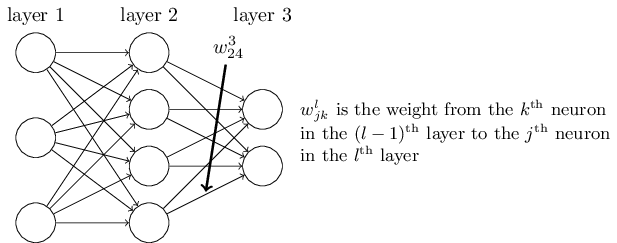
\includegraphics[width=0.9\textwidth]{images/tikz16.png}
\end{center}

\noindent 这个记号起初很笨拙，确实需要花些功夫才能掌握. 但只要稍加努力，你就会发现这个记号变得简单而自然. 这个记号的一个古怪之处是 $j$ 和 $k$ 下标的顺序. 你可能会认为用 $j$ 指代输入神经元、用 $k$ 指代输出神经元更合理，而不是像实际所做的那样反过来. 我将在下面解释这个古怪之处的原因.

我们对网络的偏置和激活值使用类似的记号. 具体来说，我们用 $b^l_j$ 表示第 $l$ 层第 $j$ 个神经元的偏置. 我们用 $a^l_j$ 表示第 $l$ 层第 $j$ 个神经元的激活值. 下图展示了这些记号的使用示例：

\begin{center}
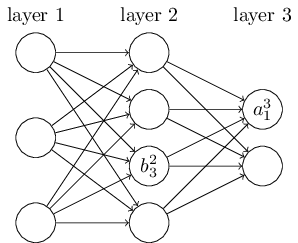
\includegraphics[width=0.9\textwidth]{images/tikz17.png}
\end{center}

\noindent 有了这些记号，第 $l$ 层第 $j$ 个神经元的激活值 $a^{l}_j$ 与第 $(l-1)$ 层的激活值通过以下方程相关联（比较上一章中的方程 (4)

\begin{align*}
\frac{1}{1+\exp(-\sum_j w_j x_j-b)} \nonumber
\end{align*}

\noindent 及周围的讨论）

\begin{equation}
a^{l}_j = \sigma\left( \sum_k w^{l}_{jk} a^{l-1}_k + b^l_j \right),
\tag{23}
\end{equation}

\noindent 其中求和是对第 $(l-1)$ 层中的所有神经元 $k$ 进行的. 为了将这个表达式改写为矩阵形式，我们为每一层 $l$ 定义一个权重矩阵 $w^l$. 权重矩阵 $w^l$ 的元素就是连接到第 $l$ 层神经元的权重，也就是说，第 $j$ 行第 $k$ 列的元素是 $w^l_{jk}$. 类似地，对于每一层 $l$，我们定义一个偏置向量 $b^l$. 你大概能猜到这是如何运作的——偏置向量的分量就是值 $b^l_j$，第 $l$ 层中的每个神经元对应一个分量. 最后，我们定义一个激活向量 $a^l$，其分量是激活值 $a^l_j$.

将 (23)

\begin{align*}
a^{l}_j = \sigma\left( \sum_k w^{l}_{jk} a^{l-1}_k + b^l_j \right) \nonumber
\end{align*}

\noindent 改写为矩阵形式所需的最后一个要素是函数向量化的概念，例如 $\sigma$. 我们在上一章简要接触过向量化，但回顾一下，其思想是我们想要将一个函数（如 $\sigma$）应用于向量 $v$ 中的每一个元素. 我们用显而易见的记号 $\sigma(v)$ 来表示这种逐元素应用函数的方式. 也就是说，$\sigma(v)$ 的分量就是 $\sigma(v)_j = \sigma(v_j)$. 举个例子，如果我们有函数 $f(x) = x^2$，那么 $f$ 的向量化形式的效果是

\begin{equation}
f\left(\left[ \begin{array}{c} 2 \\ 3 \end{array} \right] \right) = \left[ \begin{array}{c} f(2) \\ f(3) \end{array} \right] = \left[ \begin{array}{c} 4 \\ 9 \end{array} \right],
\tag{24}
\end{equation}

\noindent 也就是说，向量化的 $f$ 只是对向量的每个元素求平方.

有了这些记号，方程 (23)

\begin{align*}
a^{l}_j = \sigma\left( \sum_k w^{l}_{jk} a^{l-1}_k + b^l_j \right) \nonumber
\end{align*}

\noindent 可以改写为优美而紧凑的向量化形式

\begin{equation}
a^{l} = \sigma(w^l a^{l-1}+b^l).
\tag{25}
\end{equation}

\noindent 这个表达式为我们提供了一种更加全局的方式来思考一层中的激活值与上一层激活值之间的关系：我们只需将权重矩阵应用于激活值，然后加上偏置向量，最后应用 $\sigma$ 函数*\footnote{顺便说一下，正是这个表达式促成了前面提到的 $w^l_{jk}$ 记号中的古怪之处. 如果我们用 $j$ 来索引输入神经元、用 $k$ 来索引输出神经元，那么我们就需要将方程 (25)$a^{l} = \sigma(w^l a^{l-1}+b^l)$ 中的权重矩阵替换为其转置. 这是一个小改动，但很烦人，而且我们会失去说（和思考）``将权重矩阵应用于激活值''的那种简单明了.}. 这种全局视角通常比我们到目前为止所采用的逐个神经元的视角更容易、更简洁（而且涉及的指标更少！）. 可以把它看作一种摆脱指标地狱的方式，同时对正在发生的事情保持精确. 这个表达式在实践中也很有用，因为大多数矩阵库都提供了实现矩阵乘法、向量加法和向量化的快速方法. 事实上，上一章中的代码就隐含地使用了这个表达式来计算网络的行为.

当使用方程 (25)

\begin{align*}
a^{l} = \sigma(w^l a^{l-1}+b^l) \nonumber
\end{align*}

\noindent 来计算 $a^l$ 时，我们会在此过程中计算中间量 $z^l \equiv w^l a^{l-1}+b^l$. 这个量足够有用，值得给它起个名字：我们称 $z^l$ 为第 $l$ 层神经元的\emph{加权输入}. 我们将在本章后面大量使用加权输入 $z^l$. 方程 (25)

\begin{align*}
a^{l} = \sigma(w^l a^{l-1}+b^l) \nonumber
\end{align*}

\noindent 有时用加权输入来写，即 $a^l = \sigma(z^l)$. 还值得注意的是，$z^l$ 的分量为 $z^l_j = \sum_k w^l_{jk} a^{l-1}_k+b^l_j$，也就是说，$z^l_j$ 就是第 $l$ 层中神经元 $j$ 的激活函数的加权输入.
\sectionTitle{我们需要对代价函数做出的两条假设}{我们需要对代价函数做出的两条假设}

反向传播的目标是计算代价函数 $C$ 关于网络中任意权重 $w$ 或偏置 $b$ 的偏导数 $\partial C / \partial w$ 和 $\partial C / \partial b$. 为了让反向传播能够工作，我们需要对代价函数的形式做出两条主要假设. 不过在陈述这些假设之前，先在心里有一个代价函数的例子会很有帮助. 我们将使用上一章中的二次代价函数（参见公式 (6)

\begin{align*}
C(w,b) \equiv \frac{1}{2n} \sum_x \| y(x) - a\|^2 \nonumber
\end{align*}

\noindent ）. 用上一节的记号，二次代价具有如下形式

\begin{equation}
C = \frac{1}{2n} \sum_x \|y(x)-a^L(x)\|^2,
\tag{26}
\end{equation}

\noindent 其中：$n$ 是训练样本的总数；求和是对各个训练样本 $x$ 进行的；$y = y(x)$ 是相应的期望输出；$L$ 表示网络中的层数；而 $a^L = a^L(x)$ 是当输入为 $x$ 时网络输出的激活值向量.

好，那么为了让反向传播能够应用，我们需要对代价函数 $C$ 做出什么假设呢？我们需要的第一条假设是，代价函数可以写成对各个训练样本 $x$ 的代价函数 $C_x$ 求平均的形式 $C = \frac{1}{n} \sum_x C_x$. 二次代价函数就属于这种情况，其中单个训练样本的代价为 $C_x = \frac{1}{2} \|y-a^L \|^2$. 这条假设对于本书中我们将遇到的所有其他代价函数也同样成立.

我们需要这条假设的原因是，反向传播实际上让我们做的是计算单个训练样本的偏导数 $\partial C_x / \partial w$ 和 $\partial C_x / \partial b$. 然后我们通过对训练样本求平均来恢复 $\partial C / \partial w$ 和 $\partial C / \partial b$. 事实上，有了这条假设，我们将假定训练样本 $x$ 已经固定，并去掉 $x$ 下标，把代价 $C_x$ 写成 $C$. 我们最终会把 $x$ 放回去，但就目前而言，这是一个最好隐去不写的记号上的麻烦.

我们对代价做出的第二条假设是，它可以写成神经网络输出的函数：

\begin{center}
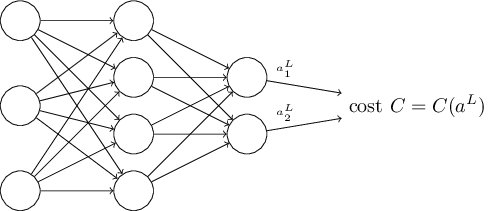
\includegraphics[width=0.9\textwidth]{images/tikz18.png}
\end{center}

\noindent 例如，二次代价函数满足这一要求，因为单个训练样本 $x$ 的二次代价可以写成

\begin{equation}
C = \frac{1}{2} \|y-a^L\|^2 = \frac{1}{2} \sum_j (y_j-a^L_j)^2,
\tag{27}
\end{equation}

\noindent 因此它是输出激活值的函数. 当然，这个代价函数也依赖于期望输出 $y$，你可能会奇怪为什么我们不把代价也看作 $y$ 的函数. 不过请记住，输入训练样本 $x$ 是固定的，因此输出 $y$ 也是一个固定的参数. 特别地，它不是我们能够通过以任何方式改变权重和偏置来修改的东西，也就是说，它不是神经网络所学习的东西. 因此，把 $C$ 看作仅依赖于输出激活值 $a^L$ 的函数是合理的，而 $y$ 仅仅是帮助定义该函数的一个参数.
\sectionTitle{Hadamard 积，$s \odot t$}{Hadamard 积，$s \odot t$}

反向传播算法基于常见的线性代数运算——比如向量加法、向量与矩阵相乘等等. 但其中有一种运算不太常用. 具体来说，假设 $s$ 和 $t$ 是两个维度相同的向量. 那么我们使用 $s \odot t$ 来表示这两个向量的\emph{逐元素}乘积. 因此 $s \odot t$ 的分量就是 $(s \odot t)_j = s_j t_j$. 举个例子，

\begin{equation}
\left[\begin{array}{c} 1 \\ 2 \end{array}\right] \odot \left[\begin{array}{c} 3 \\ 4\end{array} \right] = \left[ \begin{array}{c} 1 * 3 \\ 2 * 4 \end{array} \right] = \left[ \begin{array}{c} 3 \\ 8 \end{array} \right].
\tag{28}
\end{equation}

\noindent 这种逐元素乘法有时被称为 \emph{Hadamard 积}或 \emph{Schur 积}. 我们将称之为 Hadamard 积. 优秀的矩阵库通常会提供 Hadamard 积的快速实现，这在实现反向传播时非常方便.
\sectionTitle{反向传播背后的四个基本方程}{反向传播背后的四个基本方程}

反向传播关乎理解网络中权重和偏置的改变如何改变代价函数. 归根结底，这意味着计算偏导数 $\partial C / \partial w^l_{jk}$ 和 $\partial C / \partial b^l_j$. 但为了计算这些，我们首先引入一个中间量 $\delta^l_j$，我们称之为第 $l$ 层第 $j$ 个神经元的\emph{误差}. 反向传播将为我们提供一个计算误差 $\delta^l_j$ 的过程，然后将 $\delta^l_j$ 与 $\partial C / \partial w^l_{jk}$ 和 $\partial C / \partial b^l_j$ 联系起来.

为了理解误差是如何定义的，想象在我们的神经网络中有一个恶魔：

\begin{center}
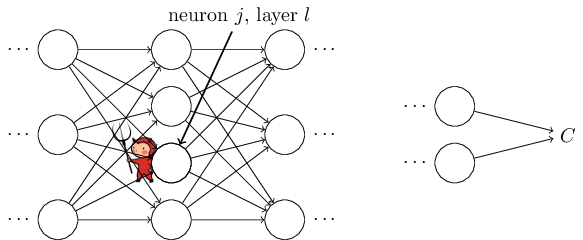
\includegraphics[width=0.9\textwidth]{images/tikz19.png}
\end{center}

\noindent 这个恶魔坐在第 $l$ 层的第 $j$ 个神经元处. 当神经元的输入到来时，恶魔干扰了神经元的运算. 它给神经元的加权输入加上一点变化 $\Delta z^l_j$，使得神经元不是输出 $\sigma(z^l_j)$，而是输出 $\sigma(z^l_j+\Delta z^l_j)$. 这个变化通过网络中后面的层传播，最终导致整体代价改变 $\frac{\partial C}{\partial z^l_j} \Delta z^l_j$.

现在，这个恶魔是一个好恶魔，它试图帮助你改善代价，也就是说，它试图找到一个使代价变小的 $\Delta z^l_j$. 假设 $\frac{\partial C}{\partial z^l_j}$ 有一个很大的值（无论是正还是负）. 那么恶魔可以通过选择 $\Delta z^l_j$ 与 $\frac{\partial C}{\partial z^l_j}$ 符号相反来大幅降低代价. 相比之下，如果 $\frac{\partial C}{\partial z^l_j}$ 接近于零，那么恶魔通过扰动加权输入 $z^l_j$ 根本无法大幅改善代价. 就恶魔所能判断的而言，这个神经元已经非常接近最优了*\footnote{当然，这只对小的变化 $\Delta z^l_j$ 成立. 我们将假设恶魔被限制只能做这样小的变化.}. 因此，从启发式的意义上说， $\frac{\partial C}{\partial z^l_j}$ 是神经元误差的一种度量.

受这个故事的启发，我们定义第 $l$ 层神经元 $j$ 的误差 $\delta^l_j$ 为

\begin{equation}
\delta^l_j \equiv \frac{\partial C}{\partial z^l_j}.
\tag{29}
\end{equation}

\noindent 按照我们通常的约定，我们用 $\delta^l$ 表示与第 $l$ 层相关的误差向量. 反向传播将为我们提供一种计算每一层的 $\delta^l$ 的方法，然后将这些误差与真正感兴趣的量为 $\partial C / \partial w^l_{jk}$ 和 $\partial C / \partial b^l_j$ 联系起来.

你可能想知道为什么恶魔改变的是加权输入 $z^l_j$. 当然，想象恶魔改变输出激活值 $a^l_j$ 会更自然，这样我们就会用 $\frac{\partial C}{\partial a^l_j}$ 作为误差的度量. 事实上，如果你这样做，结果与下面的讨论非常相似. 但事实证明，这会使反向传播的表述在代数上稍微复杂一些. 所以我们坚持用 $\delta^l_j = \frac{\partial C}{\partial z^l_j}$ 作为误差的度量*\footnote{在像 MNIST 这样的分类问题中， ``误差''一词有时被用来表示分类失败率. 例如，如果神经网络正确分类了 96.0\% 的数字，那么误差就是 4.0\%. 显然，这与我们的 $\delta$ 向量有着完全不同的含义. 在实践中，你应该不难判断在任何给定的用法中指的是哪种含义.}. \textbf{进攻计划：} 反向传播基于四个基本方程. 这些方程共同为我们提供了一种计算误差 $\delta^l$ 和代价函数梯度的方法. 我在下面陈述这四个方程. 但请注意：你不应该期望能瞬间消化这些方程. 这样的期望会导致失望. 事实上，反向传播方程如此丰富，以至于要很好地理解它们需要相当的时间和耐心，随着你逐渐深入这些方程. 好消息是，这样的耐心会得到许多倍的回报. 因此，本节的讨论仅仅是一个开始，帮助你在彻底理解这些方程的道路上前进.

以下是我们在本章后面更深入地探讨这些方程的方式预览：我将给出方程的简短证明，这有助于解释它们为什么是正确的；我们将以伪代码的算法形式重述这些方程，并看看伪代码如何实现为真正运行的 Python 代码；并且，在本章最后一节中，我们将发展一个关于反向传播方程含义的直观图景，以及某人如何可能从零开始发现它们. 在此过程中，我们将反复回到这四个基本方程，随着你理解的加深，这些方程将变得舒适，也许甚至美丽而自然. \textbf{输出层误差 $\delta^L$ 的方程：} $\delta^L$ 的分量由下式给出

\begin{equation}
\delta^L_j = \frac{\partial C}{\partial a^L_j} \sigma'(z^L_j).
\tag{BP1}
\end{equation}

\noindent 这是一个非常自然的表达式. 右边的第一项 $\partial C / \partial a^L_j$ 只是衡量代价作为第 $j$ 个输出激活值的函数变化有多快. 例如，如果 $C$ 不太依赖于某个特定的输出神经元 $j$，那么 $\delta^L_j$ 就会很小，这正是我们所期望的. 右边的第二项 $\sigma'(z^L_j)$ 衡量激活函数 $\sigma$ 在 $z^L_j$ 处变化有多快.

注意 (BP1) 中的所有内容

\begin{align*}
\delta^L_j = \frac{\partial C}{\partial a^L_j} \sigma'(z^L_j) \nonumber
\end{align*}

\noindent 都很容易计算. 特别地，我们在计算网络行为时计算 $z^L_j$，而计算 $\sigma'(z^L_j)$ 只需要很小的额外开销. $\partial C / \partial a^L_j$ 的确切形式当然取决于代价函数的形式. 然而，只要代价函数已知，计算 $\partial C / \partial a^L_j$ 应该没有什么困难. 例如，如果我们使用二次代价函数，那么 $C = \frac{1}{2} \sum_j (y_j-a^L_j)^2$，因此 $\partial C / \partial a^L_j = (a_j^L-y_j)$，这显然很容易计算.

方程 (BP1)

\begin{align*}
\delta^L_j = \frac{\partial C}{\partial a^L_j} \sigma'(z^L_j) \nonumber
\end{align*}

\noindent 是 $\delta^L$ 的逐分量表达式. 这是一个非常好的表达式，但不是我们为反向传播想要的基于矩阵的形式. 然而，很容易将方程重写为基于矩阵的形式，即

\begin{equation}
\delta^L = \nabla_a C \odot \sigma'(z^L).
\tag{BP1a}
\end{equation}

\noindent 这里， $\nabla_a C$ 被定义为一个向量，其分量为偏导数 $\partial C / \partial a^L_j$. 你可以把 $\nabla_a C$ 看作表达 $C$ 相对于输出激活值的变化率. 很容易看出方程 (BP1a)

\begin{align*}
\delta^L = \nabla_a C \odot \sigma'(z^L) \nonumber
\end{align*}

\noindent 和 (BP1)

\begin{align*}
\delta^L_j = \frac{\partial C}{\partial a^L_j} \sigma'(z^L_j) \nonumber
\end{align*}

\noindent 是等价的，因此从现在起我们将互换使用 (BP1)

\begin{align*}
\delta^L_j = \frac{\partial C}{\partial a^L_j} \sigma'(z^L_j) \nonumber
\end{align*}

\noindent 来指代这两个方程. 作为一个例子，在二次代价的情况下，我们有 $\nabla_a C = (a^L-y)$，因此 (BP1) 的完全基于矩阵的形式

\begin{align*}
\delta^L_j = \frac{\partial C}{\partial a^L_j} \sigma'(z^L_j) \nonumber
\end{align*}

\noindent 变为

\begin{equation}
\delta^L = (a^L-y) \odot \sigma'(z^L).
\tag{30}
\end{equation}

\noindent 如你所见，这个表达式中的所有内容都有很好的向量形式，并且很容易使用像 Numpy 这样的库来计算. \textbf{用下一层误差 $\delta^{l+1}$ 表示误差 $\delta^l$ 的方程：} 特别地

\begin{equation}
\delta^l = ((w^{l+1})^T \delta^{l+1}) \odot \sigma'(z^l),
\tag{BP2}
\end{equation}

\noindent 其中 $(w^{l+1})^T$ 是第 $(l+1)$ 层权重矩阵 $w^{l+1}$ 的转置. 这个方程看起来很复杂，但每个元素都有很好的解释. 假设我们知道第 $l+1$ 层的误差 $\delta^{l+1}$. 当我们应用转置权重矩阵 $(w^{l+1})^T$ 时，我们可以直观地认为这是将误差通过网络\emph{反向}移动，给我们某种第 $l$ 层输出处误差的度量. 然后我们取 Hadamard 积 $\odot \sigma'(z^l)$. 这将误差通过第 $l$ 层的激活函数反向移动，给出第 $l$ 层加权输入中的误差 $\delta^l$.

通过将 (BP2)

\begin{align*}
\delta^l = ((w^{l+1})^T \delta^{l+1}) \odot \sigma'(z^l) \nonumber
\end{align*}

\noindent 与 (BP1)

\begin{align*}
\delta^L_j = \frac{\partial C}{\partial a^L_j} \sigma'(z^L_j) \nonumber
\end{align*}

\noindent 结合，我们可以计算网络中任意层的误差 $\delta^l$. 我们首先使用 (BP1)

\begin{align*}
\delta^L_j = \frac{\partial C}{\partial a^L_j} \sigma'(z^L_j) \nonumber
\end{align*}

\noindent 计算 $\delta^L$，然后应用方程 (BP2)

\begin{align*}
\delta^l = ((w^{l+1})^T \delta^{l+1}) \odot \sigma'(z^l) \nonumber
\end{align*}

\noindent 计算 $\delta^{L-1}$，然后再次应用方程 (BP2)

\begin{align*}
\delta^l = ((w^{l+1})^T \delta^{l+1}) \odot \sigma'(z^l) \nonumber
\end{align*}

\noindent 计算 $\delta^{L-2}$，依此类推，一直反向通过网络. \textbf{代价相对于网络中任意偏置的变化率的方程：} 特别地：

\begin{equation}
\frac{\partial C}{\partial b^l_j} = \delta^l_j.
\tag{BP3}
\end{equation}

\noindent 也就是说，误差 $\delta^l_j$ \emph{恰好等于}变化率 $\partial C / \partial b^l_j$. 这是个好消息，因为 (BP1)

\begin{align*}
\delta^L_j = \frac{\partial C}{\partial a^L_j} \sigma'(z^L_j) \nonumber
\end{align*}

\noindent 和 (BP2)

\begin{align*}
\delta^l = ((w^{l+1})^T \delta^{l+1}) \odot \sigma'(z^l) \nonumber
\end{align*}

\noindent 已经告诉我们如何计算 $\delta^l_j$. 我们可以将 (BP3)

\begin{align*}
\frac{\partial C}{\partial b^l_j} = \delta^l_j \nonumber
\end{align*}

\noindent 简写为

\begin{equation}
\frac{\partial C}{\partial b} = \delta,
\tag{31}
\end{equation}

\noindent 其中 $\delta$ 被理解为在与偏置 $b$ 相同的神经元处求值. \textbf{代价相对于网络中任意权重的变化率的方程：} 特别地：

\begin{equation}
\frac{\partial C}{\partial w^l_{jk}} = a^{l-1}_k \delta^l_j.
\tag{BP4}
\end{equation}
\noindent 这告诉我们如何用已经知道如何计算的量 $\delta^l$ 和 $a^{l-1}$ 来计算偏导数 $\partial C / \partial w^l_{jk}$. 这个方程可以用一种下标更少的记号重写为

\begin{equation}
\frac{\partial C}{\partial w} = a_{\rm in} \delta_{\rm out},
\tag{32}
\end{equation}

\noindent 其中我们约定 $a_{\rm in}$ 是输入到权重 $w$ 的神经元的激活值，而 $\delta_{\rm out}$ 是从权重 $w$ 输出的神经元的误差. 放大来看，只关注权重 $w$ 以及由该权重连接的两个神经元，我们可以将其描绘为：

\begin{center}
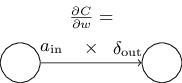
\includegraphics[width=0.9\textwidth]{images/tikz20.png}
\end{center}

\noindent 方程 (32)

\begin{align*}
\frac{\partial C}{\partial w} = a_{\rm in} \delta_{\rm out} \nonumber
\end{align*}

\noindent 的一个很好的推论是，当激活值 $a_{\rm in}$ 很小时，$a_{\rm in} \approx 0$，梯度项 $\partial C / \partial w$ 也会趋于很小. 在这种情况下，我们说该权重学习缓慢，意思是它在梯度下降过程中变化不大. 换句话说，(BP4)

\begin{align*}
\frac{\partial C}{\partial w^l_{jk}} = a^{l-1}_k \delta^l_j \nonumber
\end{align*}

\noindent 的一个推论是，从低激活值神经元输出的权重学习缓慢.

沿着这些思路，还可以从 (BP1)

\begin{align*}
\delta^L_j = \frac{\partial C}{\partial a^L_j} \sigma'(z^L_j) \nonumber
\end{align*}

\noindent -(BP4)

\begin{align*}
\frac{\partial C}{\partial w^l_{jk}} = a^{l-1}_k \delta^l_j \nonumber
\end{align*}

\noindent 中得到其他洞见. 让我们先看输出层. 考虑 (BP1)

\begin{align*}
\delta^L_j = \frac{\partial C}{\partial a^L_j} \sigma'(z^L_j) \nonumber
\end{align*}

\noindent 中的项 $\sigma'(z^L_j)$. 回想上一章中 sigmoid 函数的图像，当 $\sigma(z^L_j)$ 近似为 $0$ 或 $1$ 时，$\sigma$ 函数会变得非常平坦. 当这种情况发生时，我们将有 $\sigma'(z^L_j) \approx 0$. 因此，教训是：如果输出神经元处于低激活值（$\approx 0$）或高激活值（$\approx 1$），最后一层的权重将学习缓慢. 在这种情况下，通常说该输出神经元已经 \emph{饱和}，因此该权重已经停止学习（或学习缓慢）. 类似的评论也适用于输出神经元的偏置.

对于更早的层，我们可以得到类似的洞见. 特别地，注意 (BP2)

\begin{align*}
\delta^l = ((w^{l+1})^T \delta^{l+1}) \odot \sigma'(z^l) \nonumber
\end{align*}

\noindent 中的 $\sigma'(z^l)$ 项. 这意味着如果神经元接近饱和，$\delta^l_j$ 很可能变得很小. 而这又意味着，输入到饱和神经元的任何权重都将学习缓慢*\footnote{如果 ${w^{l+1}}^T \delta^{l+1}$ 的元素足够大，足以补偿 $\sigma'(z^l_j)$ 的微小，这个推理就不成立. 但我说的是一般趋势.}.

总结一下，我们已经了解到，如果输入神经元处于低激活值，或者输出神经元已经饱和，即处于高激活值或低激活值，那么权重将学习缓慢.

这些观察都不太令人惊讶. 不过，它们有助于改进我们对神经网络学习过程中所发生事情的心智模型. 此外，我们可以反过来利用这类推理. 这四个基本方程对任何激活函数都成立，而不仅仅是标准的 sigmoid 函数（这是因为，正如我们稍后将看到的，证明没有使用 $\sigma$ 的任何特殊性质）. 因此我们可以用这些方程来 \emph{设计} 具有特定所需学习性质的激活函数. 作为给你一个思路的例子，假设我们选择一个（非 sigmoid）激活函数 $\sigma$，使得 $\sigma'$ 始终为正，且永远不会接近零. 那将防止普通 sigmoid 神经元饱和时出现的学习减慢. 在本书后面，我们将看到对激活函数进行这种修改的例子. 牢记这四个方程 (BP1)

\begin{align*}
\delta^L_j = \frac{\partial C}{\partial a^L_j} \sigma'(z^L_j) \nonumber
\end{align*}

\noindent -(BP4)

\begin{align*}
\frac{\partial C}{\partial w^l_{jk}} = a^{l-1}_k \delta^l_j \nonumber
\end{align*}

\noindent 有助于解释为什么尝试这样的修改，以及它们可能产生什么影响.

\begin{center}
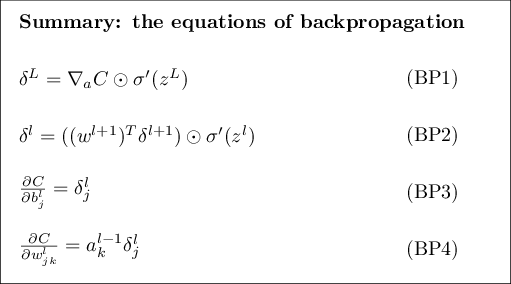
\includegraphics[width=0.9\textwidth]{images/tikz21.png}
\end{center}

\begin{exerciseBox}{习题}

\begin{itemize}

\item
\textbf{反向传播方程的另一种表述：} 我用 Hadamard 积陈述了反向传播的方程（特别是 (BP1)

\begin{align*}
\delta^L_j = \frac{\partial C}{\partial a^L_j} \sigma'(z^L_j) \nonumber
\end{align*}

和 (BP2)

\begin{align*}
\delta^l = ((w^{l+1})^T \delta^{l+1}) \odot \sigma'(z^l) \nonumber
\end{align*}

）. 如果你不熟悉 Hadamard 积，这种表述可能会让你感到困惑. 还有一种基于传统矩阵乘法的替代方法，一些读者可能会觉得有启发性. (1) 证明 (BP1)

\begin{align*}
\delta^L_j = \frac{\partial C}{\partial a^L_j} \sigma'(z^L_j) \nonumber
\end{align*}

可以重写为

\begin{equation}
\delta^L = \Sigma'(z^L) \nabla_a C,
\tag{33}
\end{equation}

其中 $\Sigma'(z^L)$ 是一个方阵，其对角元素是值 $\sigma'(z^L_j)$，非对角元素为零. 注意这个矩阵通过传统矩阵乘法作用于 $\nabla_a C$. (2) 证明 (BP2)

\begin{align*}
\delta^l = ((w^{l+1})^T \delta^{l+1}) \odot \sigma'(z^l) \nonumber
\end{align*}

可以重写为

\begin{equation}
\delta^l = \Sigma'(z^l) (w^{l+1})^T \delta^{l+1}.
\tag{34}
\end{equation}

(3) 结合观察 (1) 和 (2)，证明

\begin{equation}
\delta^l = \Sigma'(z^l) (w^{l+1})^T \ldots \Sigma'(z^{L-1}) (w^L)^T \Sigma'(z^L) \nabla_a C
\tag{35}
\end{equation}

对于熟悉矩阵乘法的读者，这个方程可能比 (BP1)

\begin{align*}
\delta^L_j = \frac{\partial C}{\partial a^L_j} \sigma'(z^L_j) \nonumber
\end{align*}

和 (BP2)

\begin{align*}
\delta^l = ((w^{l+1})^T \delta^{l+1}) \odot \sigma'(z^l) \nonumber
\end{align*}

更容易理解. 我之所以关注 (BP1)

\begin{align*}
\delta^L_j = \frac{\partial C}{\partial a^L_j} \sigma'(z^L_j) \nonumber
\end{align*}

和 (BP2)

\begin{align*}
\delta^l = ((w^{l+1})^T \delta^{l+1}) \odot \sigma'(z^l) \nonumber
\end{align*}

，是因为那种方法在数值实现上更快.

\end{itemize}

\end{exerciseBox}
\sectionTitle{四个基本方程的证明（选读）}{四个基本方程的证明（选读）}

我们现在来证明四个基本方程 (BP1)

\begin{align*}
\delta^L_j = \frac{\partial C}{\partial a^L_j} \sigma'(z^L_j) \nonumber
\end{align*}

\noindent -(BP4)

\begin{align*}
\frac{\partial C}{\partial w^l_{jk}} = a^{l-1}_k \delta^l_j \nonumber
\end{align*}

\noindent. 这四个方程都是多元微积分中链式法则的结果. 如果你对链式法则比较熟悉，那么我强烈建议你在继续阅读之前先自己尝试推导一遍.

我们从方程 (BP1)

\begin{align*}
\delta^L_j = \frac{\partial C}{\partial a^L_j} \sigma'(z^L_j) \nonumber
\end{align*}

\noindent 开始，它给出了输出误差 $\delta^L$ 的表达式. 为了证明这个方程，回忆一下根据定义

\begin{equation}
\delta^L_j = \frac{\partial C}{\partial z^L_j}.
\tag{36}
\end{equation}

\noindent 应用链式法则，我们可以将上面的偏导数重新表达为关于输出激活值的偏导数，

\begin{equation}
\delta^L_j = \sum_k \frac{\partial C}{\partial a^L_k} \frac{\partial a^L_k}{\partial z^L_j},
\tag{37}
\end{equation}

\noindent 其中求和是对输出层中所有神经元 $k$ 进行的. 当然，当 $k = j$ 时，第 $k$ 个神经元的输出激活值 $a^L_k$ 只依赖于第 $j$ 个神经元的加权输入 $z^L_j$. 因此当 $k \neq j$ 时 $\partial a^L_k / \partial z^L_j$ 为零. 于是我们可以将前面的方程简化为

\begin{equation}
\delta^L_j = \frac{\partial C}{\partial a^L_j} \frac{\partial a^L_j}{\partial z^L_j}.
\tag{38}
\end{equation}

\noindent 回忆 $a^L_j = \sigma(z^L_j)$，右边的第二项可以写成 $\sigma'(z^L_j)$，方程变为

\begin{equation}
\delta^L_j = \frac{\partial C}{\partial a^L_j} \sigma'(z^L_j),
\tag{39}
\end{equation}

\noindent 这正是 (BP1)

\begin{align*}
\delta^L_j = \frac{\partial C}{\partial a^L_j} \sigma'(z^L_j) \nonumber
\end{align*}

\noindent 的分量形式.

接下来，我们将证明 (BP2)

\begin{align*}
\delta^l = ((w^{l+1})^T \delta^{l+1}) \odot \sigma'(z^l) \nonumber
\end{align*}

\noindent，它给出了误差 $\delta^l$ 与下一层误差 $\delta^{l+1}$ 之间的关系式. 为此，我们希望将 $\delta^l_j = \partial C / \partial z^l_j$ 用 $\delta^{l+1}_k = \partial C / \partial z^{l+1}_k$ 重新表达. 我们可以利用链式法则做到这一点，

\begin{align}
\delta^l_j &= \frac{\partial C}{\partial z^l_j} \tag{40} \\ &= \sum_k \frac{\partial C}{\partial z^{l+1}_k} \frac{\partial z^{l+1}_k}{\partial z^l_j} \tag{41} \\ &= \sum_k \frac{\partial z^{l+1}_k}{\partial z^l_j} \delta^{l+1}_k, \tag{42}
\end{align}

\noindent 在最后一行中我们交换了右边的两项，并代入了 $\delta^{l+1}_k$ 的定义. 为了计算最后一行的第一项，注意到

\begin{equation}
z^{l+1}_k = \sum_j w^{l+1}_{kj} a^l_j +b^{l+1}_k = \sum_j w^{l+1}_{kj} \sigma(z^l_j) +b^{l+1}_k.
\tag{43}
\end{equation}

\noindent 求导，我们得到

\begin{equation}
\frac{\partial z^{l+1}_k}{\partial z^l_j} = w^{l+1}_{kj} \sigma'(z^l_j).
\tag{44}
\end{equation}

\noindent 代回 (42)

\begin{align*}
&= \sum_k \frac{\partial z^{l+1}_k}{\partial z^l_j} \delta^{l+1}_k \nonumber
\end{align*}

\noindent 我们得到

\begin{equation}
\delta^l_j = \sum_k w^{l+1}_{kj} \delta^{l+1}_k \sigma'(z^l_j).
\tag{45}
\end{equation}

\noindent 这正是 (BP2)

\begin{align*}
\delta^l = ((w^{l+1})^T \delta^{l+1}) \odot \sigma'(z^l) \nonumber
\end{align*}

\noindent 的分量形式.

我们要证明的最后两个方程是 (BP3)

\begin{align*}
\frac{\partial C}{\partial b^l_j} = \delta^l_j \nonumber
\end{align*}

\noindent 和 (BP4)

\begin{align*}
\frac{\partial C}{\partial w^l_{jk}} = a^{l-1}_k \delta^l_j \nonumber
\end{align*}

\noindent. 它们同样可以由链式法则推出，方式与上面两个方程的证明类似. 我把它们留给你作为练习.

\begin{exerciseBox}{练习}

\begin{itemize}

\item
证明方程 (BP3)

\begin{align*}
\frac{\partial C}{\partial b^l_j} = \delta^l_j \nonumber
\end{align*}

和 (BP4)

\begin{align*}
\frac{\partial C}{\partial w^l_{jk}} = a^{l-1}_k \delta^l_j \nonumber
\end{align*}

.

\end{itemize}

这就完成了反向传播四个基本方程的证明. 证明看起来可能很复杂. 但它实际上只是仔细应用链式法则的结果. 更简洁地说，我们可以把反向传播看作一种通过系统地应用多元微积分中的链式法则来计算代价函数梯度的方法. 反向传播本质上就是这些——其余的都是细节.

\end{exerciseBox}
\sectionTitle{反向传播算法}{反向传播算法}

反向传播方程为我们提供了一种计算代价函数梯度的方法. 让我们以算法的形式明确地写出来：

\begin{enumerate}

\item \textbf{输入 $x$：} 为输入层设置对应的激活值 $a^{1}$.

\item \textbf{前馈：} 对每个 $l = 2, 3, \ldots, L$ 计算 $z^{l} = w^l a^{l-1}+b^l$ 和 $a^{l} = \sigma(z^{l})$.

\item \textbf{输出误差 $\delta^L$：} 计算向量 $\delta^{L} = \nabla_a C \odot \sigma'(z^L)$.

\item \textbf{反向传播误差：} 对每个 $l = L-1, L-2, \ldots, 2$ 计算 $\delta^{l} = ((w^{l+1})^T \delta^{l+1}) \odot \sigma'(z^{l})$.

\item \textbf{输出：} 代价函数的梯度由 $\frac{\partial C}{\partial w^l_{jk}} = a^{l-1}_k \delta^l_j$ 和 $\frac{\partial C}{\partial b^l_j} = \delta^l_j$ 给出.

\end{enumerate}

审视这个算法，你就能明白为什么它被称为\emph{反向}传播. 我们从最后一层开始，反向计算误差向量 $\delta^l$. 我们反向遍历网络，这看起来可能有些奇怪. 但如果你想一想反向传播的证明，反向移动是代价是网络输出的函数这一事实的结果. 要理解代价如何随较早的权重和偏置变化，我们需要反复应用链式法则，从后向前逐层计算，以获得可用的表达式.

\begin{exerciseBox}{练习}

\begin{itemize}

\item \textbf{单个修改神经元的反向传播} 假设我们修改前馈网络中的单个神经元，使得该神经元的输出由 $f(\sum_j w_j x_j + b)$ 给出，其中 $f$ 是除 sigmoid 以外的某个函数. 在这种情况下，我们应该如何修改反向传播算法？

\item \textbf{线性神经元的反向传播} 假设我们在整个网络中将通常的非线性 $\sigma$ 函数替换为 $\sigma(z) = z$. 针对这种情况重写反向传播算法.

\end{itemize}

正如我上面所描述的，反向传播算法计算的是单个训练样本 $C = C_x$ 的代价函数梯度. 在实践中，通常将反向传播与随机梯度下降等学习算法结合使用，其中我们为许多训练样本计算梯度. 特别地，给定一个包含 $m$ 个训练样本的小批量，以下算法基于该小批量应用一个梯度下降学习步骤：

\begin{enumerate}

\item \textbf{输入一组训练样本}

\item \textbf{对每个训练样本 $x$：} 设置对应的输入激活值 $a^{x,1}$，并执行以下步骤：\textbf{前馈：} 对每个 $l = 2, 3, \ldots, L$ 计算 $z^{x,l} = w^l a^{x,l-1}+b^l$ 和 $a^{x,l} = \sigma(z^{x,l})$. \textbf{输出误差 $\delta^{x,L}$：} 计算向量 $\delta^{x,L} = \nabla_a C_x \odot \sigma'(z^{x,L})$. \textbf{反向传播误差：} 对每个 $l = L-1, L-2, \ldots, 2$ 计算 $\delta^{x,l} = ((w^{l+1})^T \delta^{x,l+1}) \odot \sigma'(z^{x,l})$.

\item \textbf{梯度下降：} 对每个 $l = L, L-1, \ldots, 2$ 按照规则 $w^l \rightarrow w^l-\frac{\eta}{m} \sum_x \delta^{x,l} (a^{x,l-1})^T$ 更新权重，并按照规则 $b^l \rightarrow b^l-\frac{\eta}{m} \sum_x \delta^{x,l}$ 更新偏置.

\end{enumerate}

当然，要在实践中实现随机梯度下降，你还需要一个生成训练样本小批量的外层循环，以及一个遍历多个训练轮次的外层循环. 为简单起见，我省略了这些.

\end{exerciseBox}
\sectionTitle{反向传播的代码}{反向传播的代码}

在抽象层面理解了反向传播之后，我们现在可以理解上一章中用于实现反向传播的代码了. 回想一下那一章，代码包含在 \texttt{Network} 类的 \texttt{update\_\allowbreak{}mini\_\allowbreak{}batch} 和 \texttt{backprop} 方法中. 这些方法的代码是上述算法的直接翻译. 特别地，\texttt{update\_\allowbreak{}mini\_\allowbreak{}batch} 方法通过计算当前 \texttt{mini\_\allowbreak{}batch} 训练样本的梯度来更新 \texttt{Network} 的权重和偏置：

\begin{lstlisting}
class Network(object):
...
    def update_mini_batch(self, mini_batch, eta):
        """Update the network's weights and biases by applying
        gradient descent using backpropagation to a single mini batch.
        The "mini_batch" is a list of tuples "(x, y)", and "eta"
        is the learning rate."""
        nabla_b = [np.zeros(b.shape) for b in self.biases]
        nabla_w = [np.zeros(w.shape) for w in self.weights]
        for x, y in mini_batch:
            delta_nabla_b, delta_nabla_w = self.backprop(x, y)
            nabla_b = [nb+dnb for nb, dnb in zip(nabla_b, delta_nabla_b)]
            nabla_w = [nw+dnw for nw, dnw in zip(nabla_w, delta_nabla_w)]
        self.weights = [w-(eta/len(mini_batch))*nw
                        for w, nw in zip(self.weights, nabla_w)]
        self.biases = [b-(eta/len(mini_batch))*nb
                       for b, nb in zip(self.biases, nabla_b)]

\end{lstlisting}

大部分工作由这一行完成：delta\_\allowbreak{}nabla\_\allowbreak{}b, delta\_\allowbreak{}nabla\_\allowbreak{}w = self.backprop(x, y)，它使用 backprop 方法计算出偏导数 $\partial C_x / \partial b^l_j$ 和 $\partial C_x / \partial w^l_{jk}$.backprop 方法紧密遵循上一节的算法. 有一个小的改动——我们使用了一种略微不同的层索引方式. 这一改动是为了利用 Python 的一个特性，即使用负数列表索引从列表末尾向前计数，例如，l[-3] 是列表 l 中的倒数第三个元素. 下面是 backprop 的代码，以及一些辅助函数，用于计算 $\sigma$ 函数、导数 $\sigma'$ 以及代价函数的导数. 有了这些内容，你应该能够以自包含的方式理解代码. 如果有什么地方让你困惑，查阅代码的原始描述（以及完整清单）可能会有所帮助.

\begin{lstlisting}
class Network(object):
...
   def backprop(self, x, y):
        """Return a tuple "(nabla_b, nabla_w)" representing the
        gradient for the cost function C_x.  "nabla_b" and
        "nabla_w" are layer-by-layer lists of numpy arrays, similar
        to "self.biases" and "self.weights"."""
        nabla_b = [np.zeros(b.shape) for b in self.biases]
        nabla_w = [np.zeros(w.shape) for w in self.weights]
        # feedforward
        activation = x
        activations = [x] # list to store all the activations, layer by layer
        zs = [] # list to store all the z vectors, layer by layer
        for b, w in zip(self.biases, self.weights):
            z = np.dot(w, activation)+b
            zs.append(z)
            activation = sigmoid(z)
            activations.append(activation)
        # backward pass
        delta = self.cost_derivative(activations[-1], y) * \
            sigmoid_prime(zs[-1])
        nabla_b[-1] = delta
        nabla_w[-1] = np.dot(delta, activations[-2].transpose())
        # Note that the variable l in the loop below is used a little
        # differently to the notation in Chapter 2 of the book.  Here,
        # l = 1 means the last layer of neurons, l = 2 is the
        # second-last layer, and so on.  It's a renumbering of the
        # scheme in the book, used here to take advantage of the fact
        # that Python can use negative indices in lists.
        for l in xrange(2, self.num_layers):
            z = zs[-l]
            sp = sigmoid_prime(z)
            delta = np.dot(self.weights[-l+1].transpose(), delta) * sp
            nabla_b[-l] = delta
            nabla_w[-l] = np.dot(delta, activations[-l-1].transpose())
        return (nabla_b, nabla_w)

...

    def cost_derivative(self, output_activations, y):
        """Return the vector of partial derivatives \partial C_x /
        \partial a for the output activations."""
        return (output_activations-y)

def sigmoid(z):
    """The sigmoid function."""
    return 1.0/(1.0+np.exp(-z))

def sigmoid_prime(z):
    """Derivative of the sigmoid function."""
    return sigmoid(z)*(1-sigmoid(z))

\end{lstlisting}

\begin{exerciseBox}{习题}

\begin{itemize}

\item \textbf{基于小批量的完全矩阵化反向传播方法} 我们的随机梯度下降实现是在一个小批量中循环遍历训练样本. 可以修改反向传播算法，使其同时计算一个小批量中所有训练样本的梯度. 其思路是，不从单个输入向量 $x$ 开始，而是从一个矩阵 $X = [x_1 x_2 \ldots x_m]$ 开始，其列是小批量中的向量. 我们通过乘以权重矩阵、加上适当的偏置项矩阵，并在各处应用 S 型函数来进行前向传播. 我们以类似的方式进行反向传播. 请明确写出这种反向传播算法方法的伪代码. 修改 \texttt{network.py} 使其使用这种完全矩阵化的方法. 这种方法的优势在于它充分利用了现代线性代数库. 因此，它可能比循环遍历小批量快得多.（例如，在我的笔记本电脑上，当运行在上一章所考虑的那种 MNIST 分类问题上时，加速大约为两倍.）在实践中，所有严肃的反向传播库都使用这种完全矩阵化的方法或某种变体.

\end{itemize}

\end{exerciseBox}
\sectionTitle{反向传播究竟快在哪里？}{反向传播究竟快在哪里？}

反向传播究竟快在哪里？为了回答这个问题，让我们考虑另一种计算梯度的方式. 想象一下神经网络研究的早期. 也许是 20 世纪 50 年代或 60 年代，而你是世界上第一个想到用梯度下降来学习的人！但要让这个想法奏效，你需要一种计算代价函数梯度的方法. 你回想起自己的微积分知识，决定看看能否用链式法则来计算梯度. 但摆弄了一阵之后，代数式看起来变得很复杂，你感到气馁. 于是你尝试寻找另一种方式. 你决定把代价仅仅看作权重的函数 $C = C(w)$（我们稍后再回到偏置的问题）. 你把权重编号为 $w_1, w_2, \ldots$，并想对某个特定的权重 $w_j$ 计算 $\partial C / \partial w_j$. 一个显而易见的方法是使用近似

\begin{equation}
\frac{\partial C}{\partial w_{j}} \approx \frac{C(w+\epsilon e_j)-C(w)}{\epsilon},
\tag{46}
\end{equation}

\noindent 其中 $\epsilon > 0$ 是一个很小的正数，而 $e_j$ 是第 $j$ 个方向上的单位向量. 换句话说，我们可以通过计算 $w_j$ 两个略有不同的取值下的代价 $C$，然后应用方程 (46)

\begin{align*}
\frac{\partial C}{\partial w_{j}} \approx \frac{C(w+\epsilon e_j)-C(w)}{\epsilon} \nonumber
\end{align*}

\noindent 来估计 $\partial C / \partial w_j$. 同样的想法可以让我们计算关于偏置的偏导数 $\partial C / \partial b$.

这种方法看起来很有前途. 它在概念上很简单，而且实现起来极其容易，只需要几行代码. 当然，它看起来比用链式法则计算梯度的想法更有前途得多！

不幸的是，尽管这种方法看起来很有前途，但当你实现代码时，它却变得极其缓慢. 要理解其中的原因，想象我们的网络有一百万个权重. 那么对于每一个不同的权重 $w_j$，我们都需要计算 $C(w+\epsilon e_j)$ 才能算出 $\partial C / \partial w_j$. 这意味着为了计算梯度，我们需要计算代价函数一百万次，这要求（对每个训练样本）进行一百万次通过网络的前向传播. 我们还需要计算 $C(w)$，所以总共是一百万零一次通过网络的前向传播.

反向传播的巧妙之处在于，它使我们能够仅用一次通过网络的前向传播，随后一次通过网络的后向传播，就同时计算\emph{所有}偏导数 $\partial C / \partial w_j$. 粗略地说，后向传播的计算代价与前向传播大致相同*\footnote{这应该是合理的，但要做出严谨的陈述还需要一些分析. 它之所以合理，是因为前向传播中主要的计算代价是乘以权重矩阵，而在后向传播中则是乘以权重矩阵的转置. 这些操作显然具有相似的计算代价.}. 因此反向传播的总代价大致相当于仅进行两次通过网络的前向传播. 把它与基于 (46)

\begin{align*}
\frac{\partial C}{\partial w_{j}} \approx \frac{C(w+\epsilon e_j)-C(w)}{\epsilon} \nonumber
\end{align*}

\noindent 的方法所需的一百万零一次前向传播相比！因此，尽管反向传播表面上看起来比基于 (46)

\begin{align*}
\frac{\partial C}{\partial w_{j}} \approx \frac{C(w+\epsilon e_j)-C(w)}{\epsilon} \nonumber
\end{align*}

\noindent 的方法更复杂，但它实际上要快得多得多.

这种加速在 1986 年首次得到充分认识，它极大地扩展了神经网络能够解决的问题范围. 这反过来又引发了人们使用神经网络的热潮. 当然，反向传播并非万能药. 即使在 20 世纪 80 年代末，人们也遇到了极限，尤其是在尝试用反向传播训练深度神经网络，即具有许多隐藏层的网络时. 在本书后面，我们将看到现代计算机和一些巧妙的新想法如何使利用反向传播训练这样的深度神经网络成为可能.
\sectionTitle{反向传播：整体图景}{反向传播：整体图景}

正如我所解释的，反向传播呈现出两个谜团. 首先，这个算法究竟在做什么？我们已经建立了一幅误差从输出端反向传播的图景. 但是，我们能否更深入一些，对我们在进行所有这些矩阵和向量乘法时究竟发生了什么建立起更多的直觉？第二个谜团是，最初怎么会有人发现反向传播？遵循一个算法的步骤，甚至遵循该算法有效的证明，这是一回事. 但这并不意味着你对问题的理解如此透彻，以至于你本来能够首先发现这个算法. 是否存在一条合理的推理路线，能够引导你发现反向传播算法？在本节中，我将探讨这两个谜团.

为了增进我们对这个算法在做什么的直觉，让我们想象我们对网络中的某个权重 $w^l_{jk}$ 做了一个微小的改变 $\Delta w^l_{jk}$：

\begin{center}
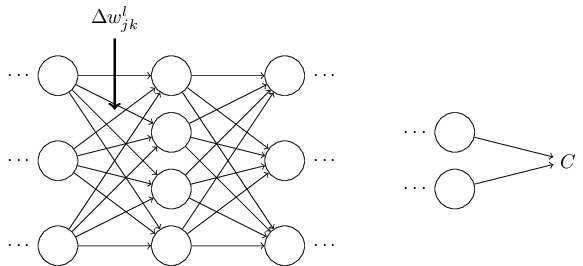
\includegraphics[width=0.9\textwidth]{images/tikz22.png}
\end{center}

\noindent 权重的这个改变将导致相应神经元的输出激活值发生变化：

\begin{center}
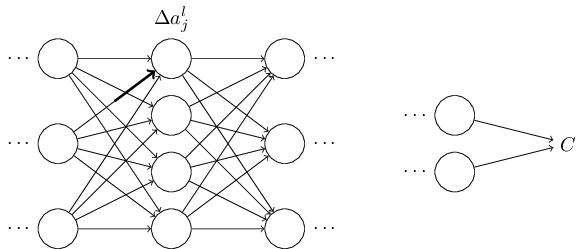
\includegraphics[width=0.9\textwidth]{images/tikz23.png}
\end{center}

\noindent 这反过来又会导致下一层中所有激活值发生变化：

\begin{center}
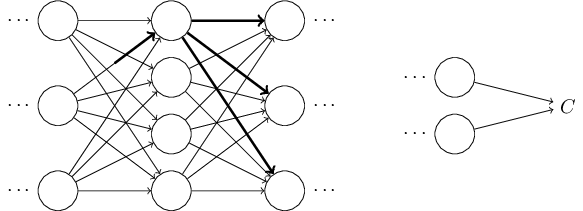
\includegraphics[width=0.9\textwidth]{images/tikz24.png}
\end{center}

\noindent 这些变化又会依次导致下一层发生变化，然后是再下一层，如此一直下去，直到导致最终层发生变化，进而导致代价函数发生变化：

\begin{center}
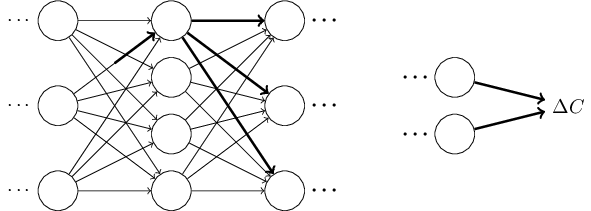
\includegraphics[width=0.9\textwidth]{images/tikz25.png}
\end{center}

\noindent 代价的变化 $\Delta C$ 与权重的变化 $\Delta w^l_{jk}$ 之间的关系由以下方程给出

\begin{equation}
\Delta C \approx \frac{\partial C}{\partial w^l_{jk}} \Delta w^l_{jk}.
\tag{47}
\end{equation}

\noindent 这表明，计算 $\frac{\partial C}{\partial w^l_{jk}}$ 的一种可能方法是仔细追踪 $w^l_{jk}$ 的微小变化如何传播并导致 $C$ 的微小变化. 如果我们能做到这一点，并且在此过程中小心地将一切都用易于计算的量来表示，那么我们就应该能够计算出 $\partial C / \partial w^l_{jk}$.

让我们试着来实现这一点. 变化 $\Delta w^l_{jk}$ 导致第 $l$ 层中第 $j$ 个神经元的激活值发生微小变化 $\Delta a^{l}_j$. 这个变化由下式给出

\begin{equation}
\Delta a^l_j \approx \frac{\partial a^l_j}{\partial w^l_{jk}} \Delta w^l_{jk}.
\tag{48}
\end{equation}

\noindent 激活值的变化 $\Delta a^l_{j}$ 将导致下一层，即第 $(l+1)$ 层中\emph{所有}激活值发生变化. 我们将集中讨论其中仅仅一个激活值受到影响的方式，比如 $a^{l+1}_q$，

\begin{center}
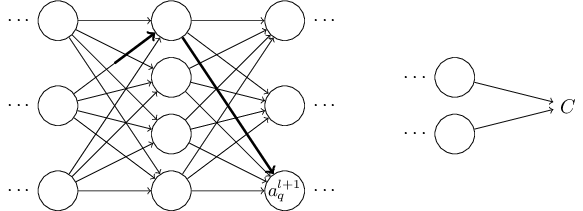
\includegraphics[width=0.9\textwidth]{images/tikz26.png}
\end{center}

\noindent 事实上，它将导致以下变化：

\begin{equation}
\Delta a^{l+1}_q \approx \frac{\partial a^{l+1}_q}{\partial a^l_j} \Delta a^l_j.
\tag{49}
\end{equation}

\noindent 代入方程 (48) 中的表达式

\begin{align*}
\Delta a^l_j \approx \frac{\partial a^l_j}{\partial w^l_{jk}} \Delta w^l_{jk} \nonumber
\end{align*}

\noindent，我们得到：

\begin{equation}
\Delta a^{l+1}_q \approx \frac{\partial a^{l+1}_q}{\partial a^l_j} \frac{\partial a^l_j}{\partial w^l_{jk}} \Delta w^l_{jk}.
\tag{50}
\end{equation}

\noindent 当然，变化 $\Delta a^{l+1}_q$ 又会依次导致下一层中激活值的变化. 事实上，我们可以想象一条从 $w^l_{jk}$ 到 $C$ 贯穿整个网络的路径，其中每一次激活值的变化都会导致下一个激活值的变化，最后导致输出端代价的变化. 如果这条路径经过激活值 $a^l_j, a^{l+1}_q, \ldots, a^{L-1}_n, a^L_m$，那么得到的表达式是

\begin{equation}
\Delta C \approx \frac{\partial C}{\partial a^L_m} \frac{\partial a^L_m}{\partial a^{L-1}_n} \frac{\partial a^{L-1}_n}{\partial a^{L-2}_p} \ldots \frac{\partial a^{l+1}_q}{\partial a^l_j} \frac{\partial a^l_j}{\partial w^l_{jk}} \Delta w^l_{jk},
\tag{51}
\end{equation}

\noindent 也就是说，对于我们经过的每一个额外的神经元，我们都获得了一个 $\partial a / \partial a$ 类型的项，以及最后的 $\partial C/\partial a^L_m$ 项. 这代表了由于沿着这条特定路径通过网络时激活值的变化所引起的 $C$ 的变化. 当然，$w^l_{jk}$ 的变化可以通过许多路径传播并影响代价，而我们只考虑了单条路径. 为了计算 $C$ 的总变化，我们似乎应该对权重和最终代价之间所有可能的路径求和，即

\begin{equation}
\Delta C \approx \sum_{mnp\ldots q} \frac{\partial C}{\partial a^L_m} \frac{\partial a^L_m}{\partial a^{L-1}_n} \frac{\partial a^{L-1}_n}{\partial a^{L-2}_p} \ldots \frac{\partial a^{l+1}_q}{\partial a^l_j} \frac{\partial a^l_j}{\partial w^l_{jk}} \Delta w^l_{jk},
\tag{52}
\end{equation}

\noindent 其中我们对路径上所有可能的中间神经元选择进行了求和. 与 (47) 比较

\begin{align*}
\Delta C \approx \frac{\partial C}{\partial w^l_{jk}} \Delta w^l_{jk} \nonumber
\end{align*}

\noindent 我们看到

\begin{equation}
\frac{\partial C}{\partial w^l_{jk}} = \sum_{mnp\ldots q} \frac{\partial C}{\partial a^L_m} \frac{\partial a^L_m}{\partial a^{L-1}_n} \frac{\partial a^{L-1}_n}{\partial a^{L-2}_p} \ldots \frac{\partial a^{l+1}_q}{\partial a^l_j} \frac{\partial a^l_j}{\partial w^l_{jk}}.
\tag{53}
\end{equation}

\noindent 现在，方程 (53)

\begin{align*}
\frac{\partial C}{\partial w^l_{jk}} = \sum_{mnp\ldots q} \frac{\partial C}{\partial a^L_m} \frac{\partial a^L_m}{\partial a^{L-1}_n} \frac{\partial a^{L-1}_n}{\partial a^{L-2}_p} \ldots \frac{\partial a^{l+1}_q}{\partial a^l_j} \frac{\partial a^l_j}{\partial w^l_{jk}} \nonumber
\end{align*}

\noindent 看起来很复杂. 然而，它有一个很好的直观解释. 我们正在计算 $C$ 相对于网络中某个权重的变化率. 这个方程告诉我们的是，网络中两个神经元之间的每条边都关联着一个速率因子，它就是一个神经元的激活值相对于另一个神经元激活值的偏导数. 从第一个权重到第一个神经元的边有一个速率因子 $\partial a^{l}_j / \partial w^l_{jk}$. 一条路径的速率因子就是沿着该路径的速率因子的乘积. 而总的变化率 $\partial C / \partial w^l_{jk}$ 就是从初始权重到最终代价的所有路径的速率因子之和. 这个过程在此处针对单条路径进行了说明：

\begin{center}
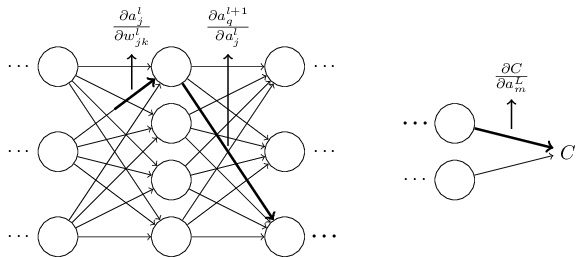
\includegraphics[width=0.9\textwidth]{images/tikz27.png}
\end{center}

\noindent 到目前为止，我提供的是一种启发式论证，一种思考当你扰动网络中的权重时发生了什么的方式. 让我勾勒出一条你可以用来进一步发展这个论证的思路. 首先，你可以推导出方程 (53) 中所有各个偏导数的显式表达式

\begin{align*}
\frac{\partial C}{\partial w^l_{jk}} = \sum_{mnp\ldots q} \frac{\partial C}{\partial a^L_m} \frac{\partial a^L_m}{\partial a^{L-1}_n} \frac{\partial a^{L-1}_n}{\partial a^{L-2}_p} \ldots \frac{\partial a^{l+1}_q}{\partial a^l_j} \frac{\partial a^l_j}{\partial w^l_{jk}} \nonumber
\end{align*}

\noindent. 用一点微积分很容易做到这一点. 完成之后，你可以尝试弄清楚如何将所有对指标的求和写成矩阵乘法. 事实证明这很繁琐，需要一些毅力，但不需要非凡的洞察力. 在做完所有这些，然后尽可能简化之后，你会发现你最终得到的正是反向传播算法！因此，你可以把反向传播算法看作提供了一种计算所有这些路径的速率因子之和的方法. 或者，稍微换个说法，反向传播算法是一种巧妙的方法，用于追踪权重（和偏置）的微小扰动在通过网络传播、到达输出、进而影响代价的过程.

现在，我不打算在这里把这一切都过一遍. 这很混乱，需要相当小心才能处理完所有细节. 如果你愿意接受挑战，你可能会喜欢尝试一下. 即使不愿意，我也希望这条思路能让你对反向传播所取得的成就有所领悟.

那么另一个谜团呢——反向传播最初是如何被发现的？事实上，如果你遵循我刚才勾勒的方法，你会发现反向传播的一个证明. 不幸的是，这个证明比我在本章前面描述的那个要长得多，也复杂得多. 那么，那个简短（但更神秘）的证明是如何被发现的呢？当你写出长证明的所有细节时，你会发现，事后看来，有几个明显的简化就摆在眼前. 你做出那些简化，得到一个更短的证明，并把它写出来. 然后又有几个明显的简化跳出来. 于是你再次重复. 经过几次迭代后得到的结果就是我们之前看到的证明*\footnote{这里需要一个巧妙的步骤. 在方程 (53) $\frac{\partial C}{\partial w^l_{jk}} = \sum_{mnp\ldots q} \frac{\partial C}{\partial a^L_m} \frac{\partial a^L_m}{\partial a^{L-1}_n} \frac{\partial a^{L-1}_n}{\partial a^{L-2}_p} \ldots \frac{\partial a^{l+1}_q}{\partial a^l_j} \frac{\partial a^l_j}{\partial w^l_{jk}}$ 中，中间变量是像 $a_q^{l+1}$ 这样的激活值. 巧妙的想法是改用加权输入，比如 $z^{l+1}_q$，作为中间变量. 如果你没有这个想法，而是继续使用激活值 $a^{l+1}_q$，你得到的证明结果会比本章前面给出的证明稍微复杂一些.}——简短，但有些晦涩，因为所有指向其构造的路标都被移除了！当然，我是在请求你相信我这一点，但早期证明的起源确实没有什么大的谜团. 它只是大量艰苦的工作，简化了我在本节中勾勒的证明.
